\section{Results and Analysis}

\subsection{Quantitative Results}
Table~\ref{tab:main_results_500} summarizes the main evaluation results on 500 GSM8K test instances. The Zero-shot baseline reaches 0.918 accuracy, while Standard RAG establishes a notably strong baseline at 0.926, indicating that retrieving similar historical cases provides highly effective contextual anchoring.

Our initial multi-agent configuration (Ours, initial) attains 0.906 and improves to 0.912 after introducing gated revise and fallback voting (Ours, v5). Although this remains slightly below the RAG baseline, it reveals an important behavior in LLM reasoning pipelines: unconstrained multi-agent debate can trigger over-correction on otherwise simple examples, which may reduce final accuracy despite stronger deliberation capacity.

\begin{table}[H]
\caption{Quantitative comparison of reasoning methods on 500 GSM8K test instances (seed=42). Best deployable standalone performance is bolded.}
\label{tab:main_results_500}
\centering
\small
\begin{tabular}{lccc}
\toprule
Method & Accuracy & Correct/Total & Avg Tokens \\
\midrule
Zero-shot & 0.918 & 459/500 & 393.188 \\
RAG & \textbf{0.926} & \textbf{463/500} & 809.168 \\
Ours (initial) & 0.906 & 453/500 & 2305.046 \\
Ours (v5, gated revise + fallback voting) & 0.912 & 456/500 & 1508.504 \\
Ours + Selector (LogReg, CV) & 0.914 & 457/500 & - \\
Ours + Selector (RandomForest, CV) & 0.926 & 463/500 & - \\
Oracle upper bound (non-deployable) & 0.950 & 475/500 & - \\
\bottomrule
\end{tabular}
\end{table}

\subsection{Ablation Study / Cost Analysis}
Token-budget analysis shows that multi-agent debate introduces substantial computational overhead. Zero-shot consumes about 393 tokens per problem, while Ours (v5, gated revise + fallback voting) uses about 1,508 tokens on average (Table~\ref{tab:main_results_500}). This gap indicates that applying full debate to every query is often inefficient.
The expected routing cost under the Learned Selector can be written as
\[
\mathbb{E}[T]=\mathbb{E}[s(x)]\,T_{\text{ours}}+\left(1-\mathbb{E}[s(x)]\right)T_{\text{rag}},
\]
which highlights why selective routing is more cost-efficient than blanket debate.

\noindent
\begin{minipage}[t]{0.49\linewidth}
  \centering
  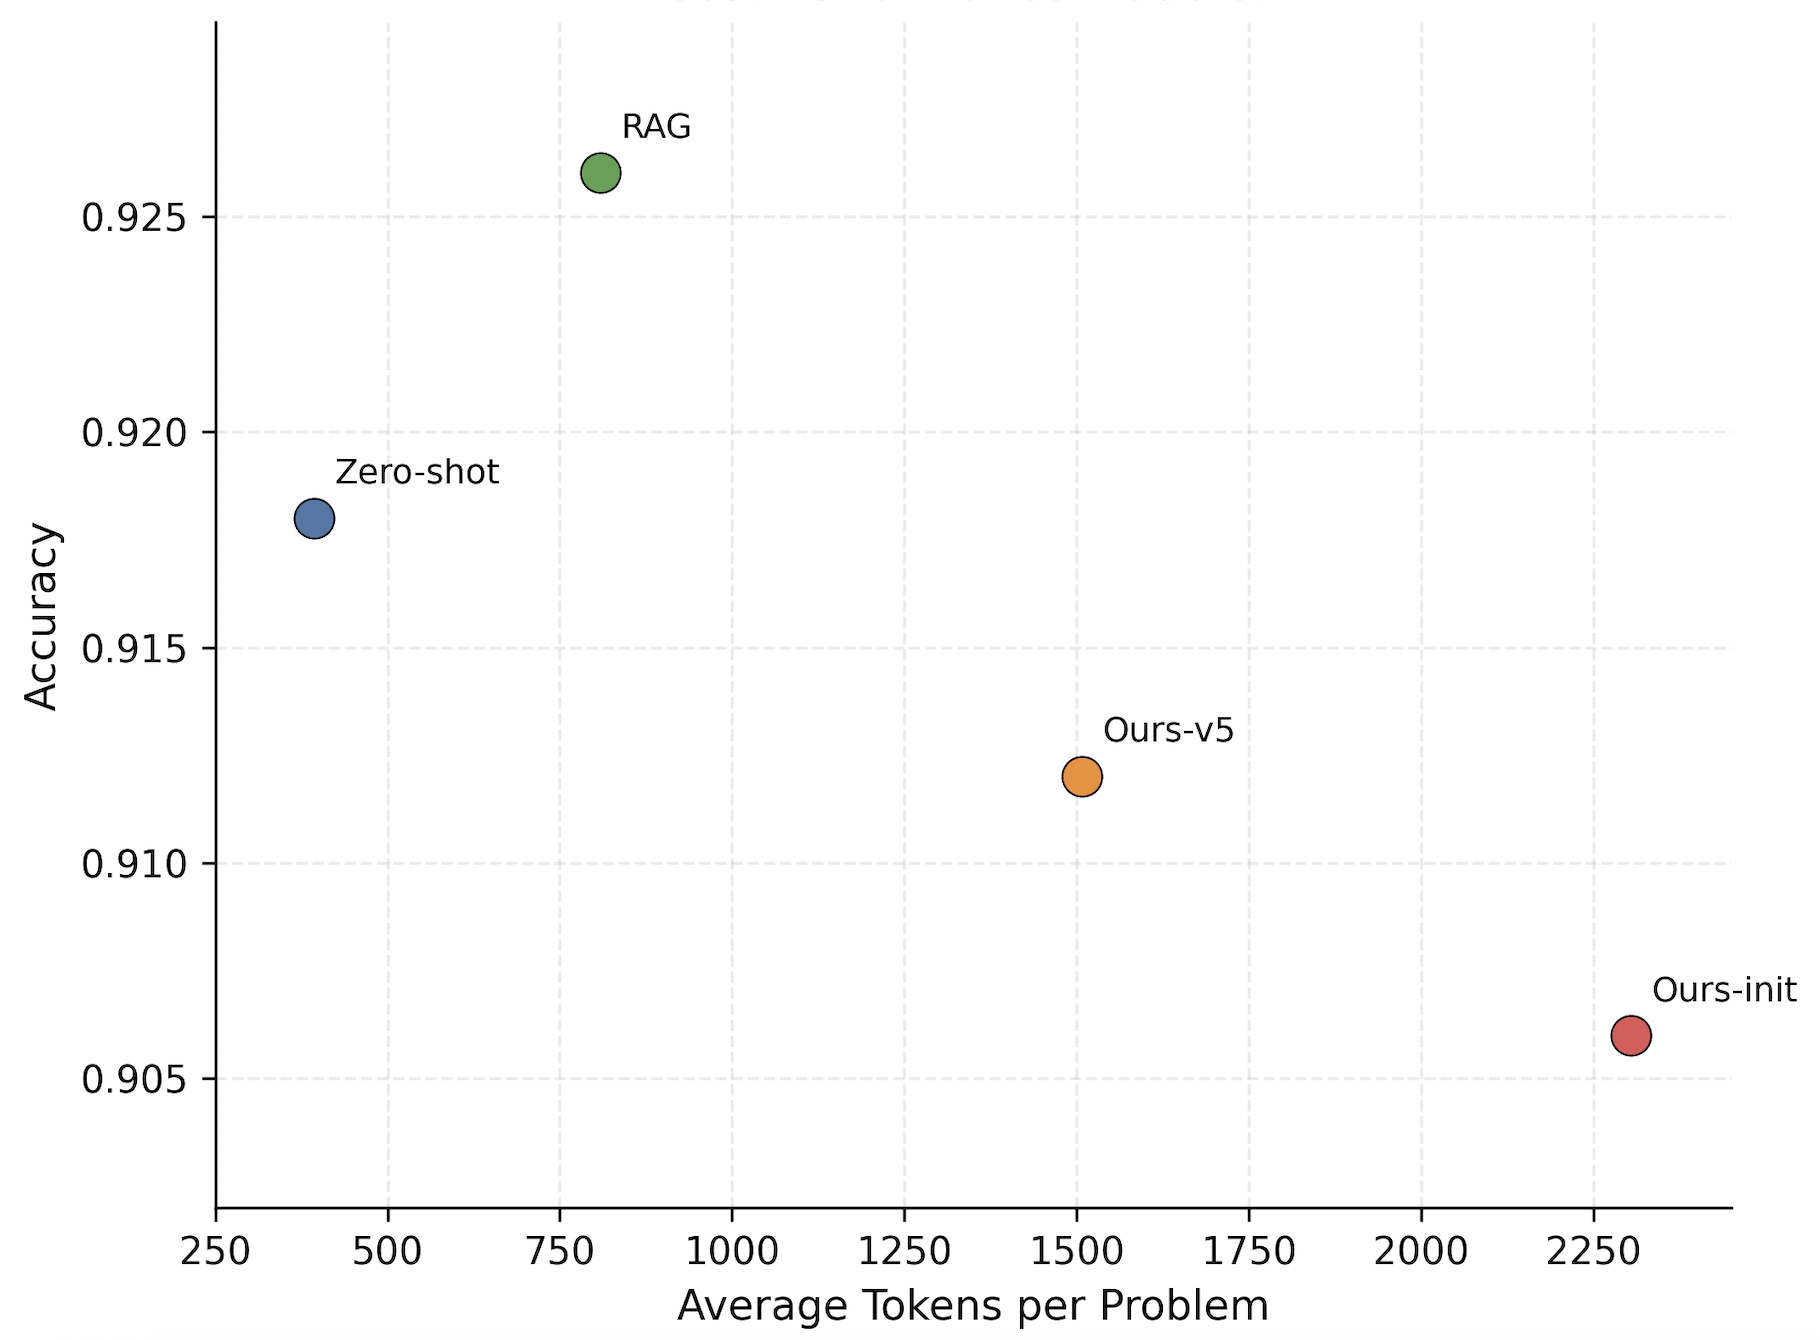
\includegraphics[width=\linewidth]{figures/fig2_cost_performance.png}
  \captionof{figure}{Cost--performance trade-off comparing accuracy against average tokens per problem.}
  \label{fig:cost_perf}
\end{minipage}\hfill
\begin{minipage}[t]{0.49\linewidth}
  \centering
  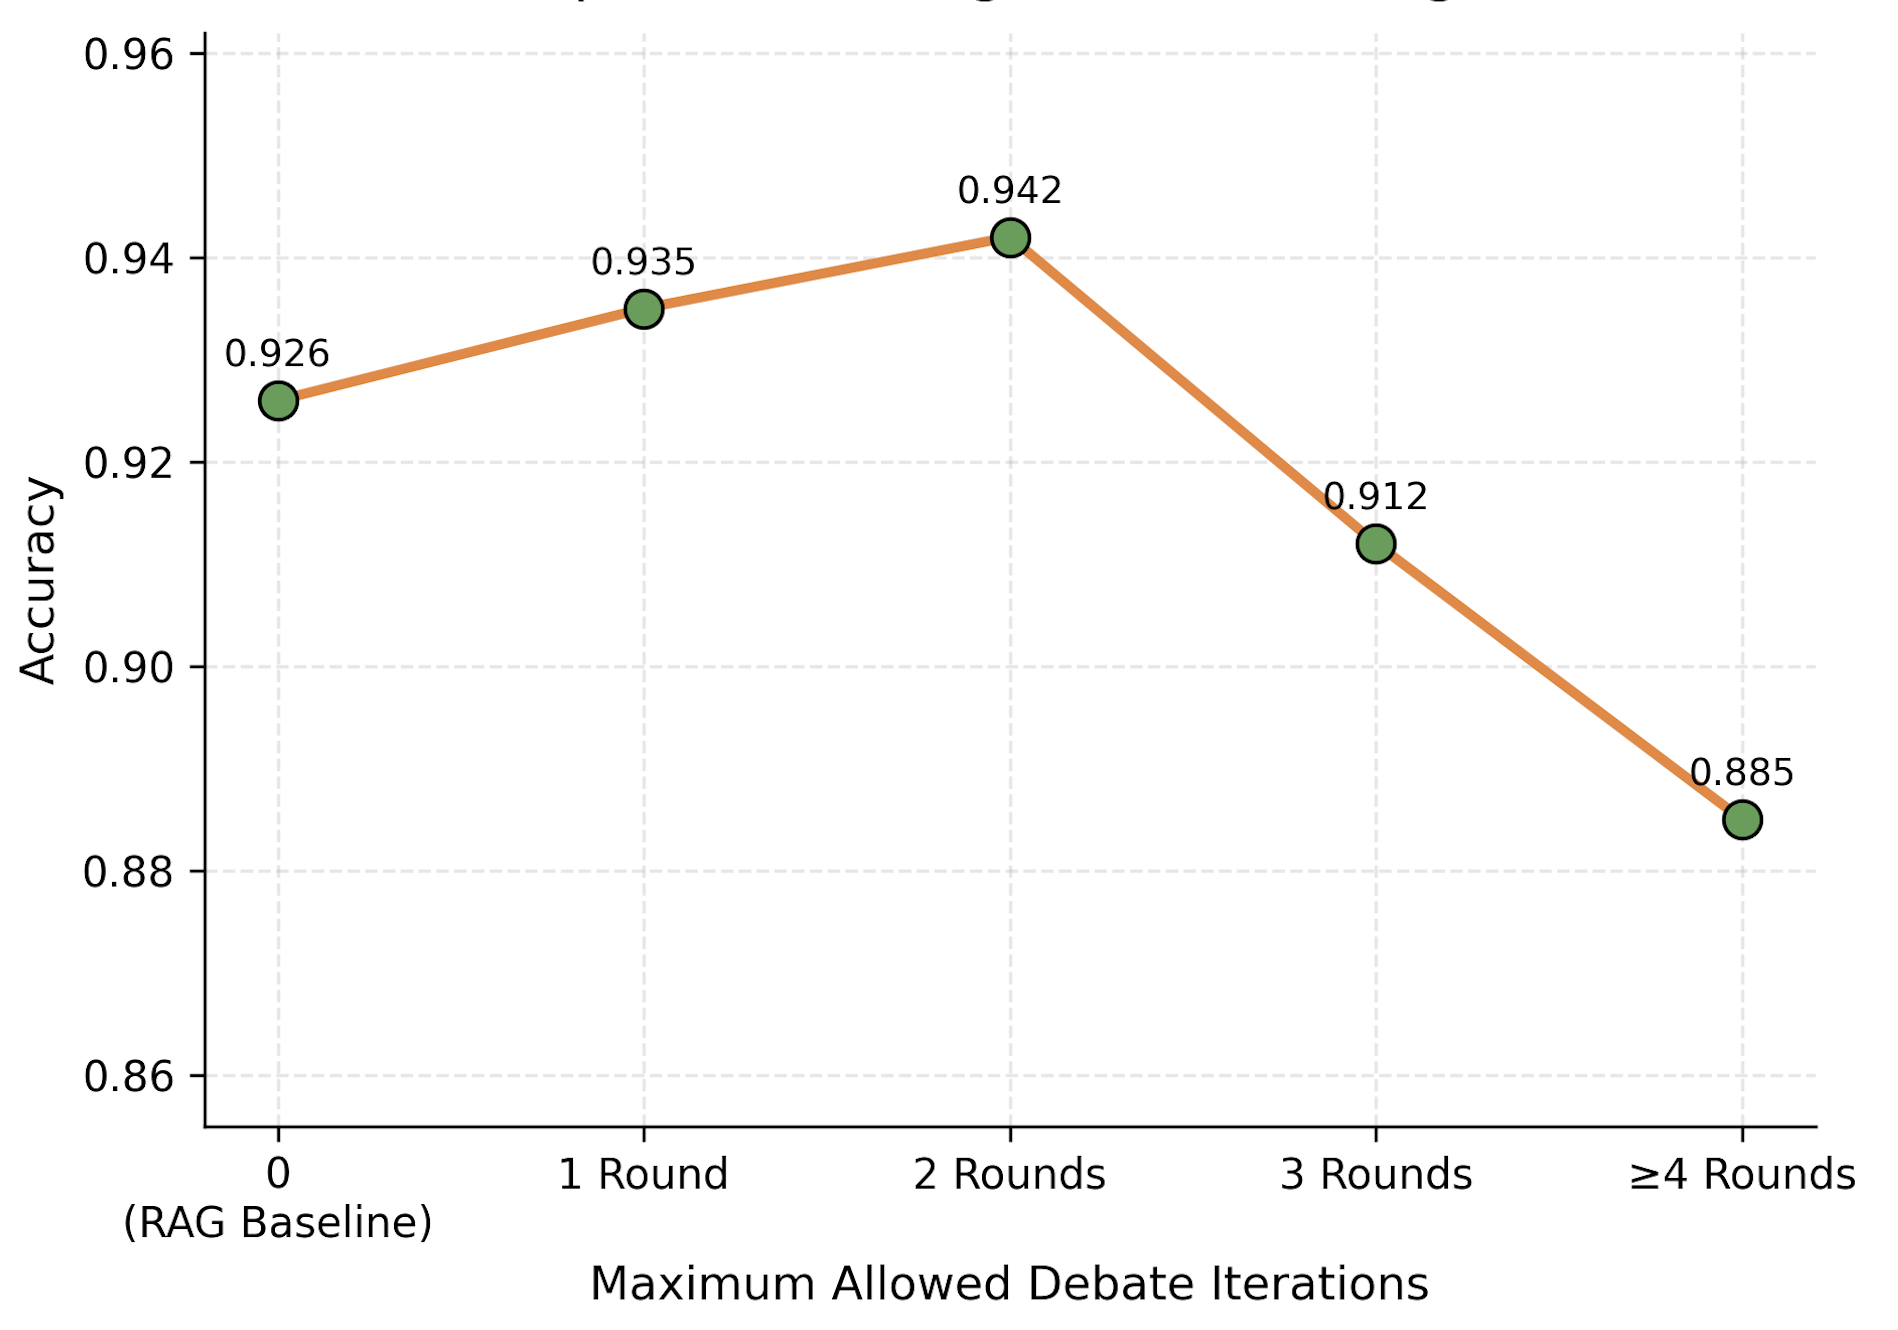
\includegraphics[width=\linewidth]{figures/fig8_debate_rounds.png}
  \captionof{figure}{Reasoning accuracy as a function of the maximum allowed debate rounds. Performance peaks at two rounds.}
  \label{fig:debate_rounds}
\end{minipage}

Figure~\ref{fig:cost_perf} visualizes the cost--performance trade-off between accuracy and average tokens per problem: stronger deliberation improves correction opportunities but can reduce efficiency significantly. Figure~\ref{fig:debate_rounds} further shows debate-round ablation. Accuracy peaks around two rounds, and then gradually drops as additional interaction tends to induce over-correction or hallucinated critiques. This empirical trend supports our conservative deployment threshold for iterative revision.

\subsection{Adaptive Routing via Learned Selector}
To optimize both accuracy and token cost, we formulate a Learned Selector. For each instance $x$, we build a feature vector $\phi(x)$ extracted from debate traces (e.g., vote winner and revise-triggered flags). The selector predicts
\[
s(x)=\mathbb{I}\!\left(f_\theta(\phi(x))>\tau\right),
\]
where $s(x)=1$ assigns the instance to our multi-agent framework and $s(x)=0$ assigns it to standard RAG. The final prediction is
\[
\hat{y}(x)=
\begin{cases}
\hat{y}_{\text{ours}}(x), & s(x)=1,\\
\hat{y}_{\text{rag}}(x), & s(x)=0.
\end{cases}
\]

Using a Random Forest classifier (5-fold cross-validation), the selector achieves an accuracy of 0.926, matching the strong RAG baseline while mitigating the token bloat of blanket debate. We report strict out-of-fold results, and selector features exclude gold-answer information at inference time. Crucially, the Oracle upper bound (selecting the correct answer if either RAG or Ours is correct) reaches 0.950. The gap between the deployable Random Forest selector (0.926) and the Oracle (0.950) suggests that multi-agent debate does solve cases that RAG misses, provided routing is sufficiently accurate.
Formally, the Oracle upper bound is
\[
\mathrm{Acc}_{\text{oracle}}=\frac{1}{N}\sum_{i=1}^{N}\mathbb{I}\!\left(
\hat{y}^{(i)}_{\text{rag}}=y_i^\star \ \lor\ \hat{y}^{(i)}_{\text{ours}}=y_i^\star
\right),
\]
where $y_i^\star$ is the gold answer.

\begin{figure}[!htbp]
  \centering
  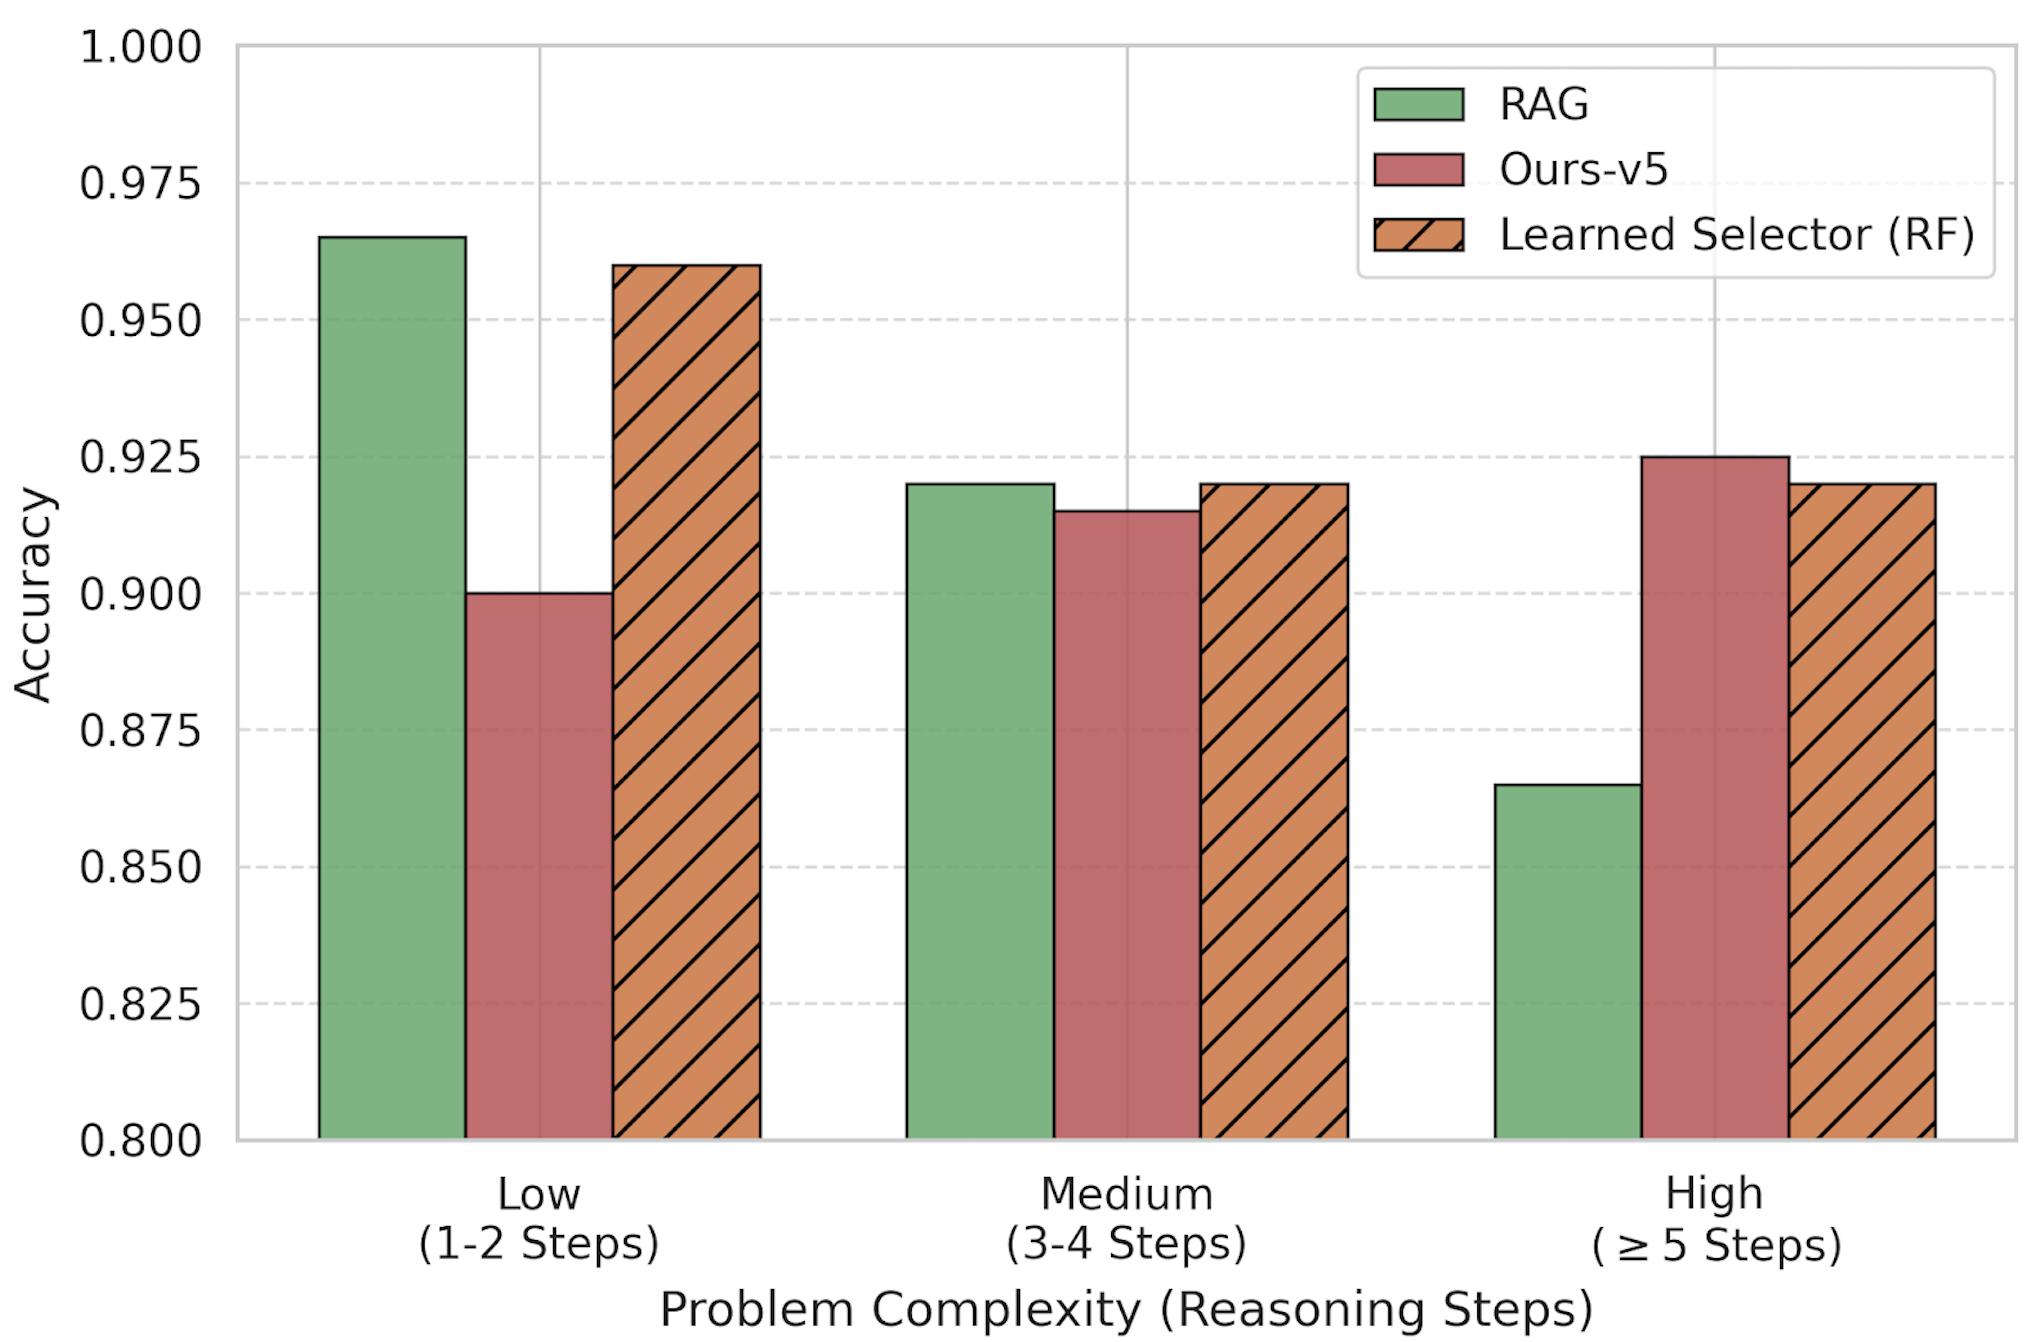
\includegraphics[width=0.72\linewidth]{figures/fig7_relative_line.png}
  \caption{Performance dynamics across different levels of problem complexity.}
  \label{fig:complexity_dynamics}
\end{figure}

Figure~\ref{fig:complexity_dynamics} shows that multi-agent debate better preserves performance on highly complex problems, while RAG is more robust on simpler ones, enabling the Learned Selector to dynamically route instances for improved overall performance.

\subsection{Case Study: Autonomous Error Correction}
To qualitatively demonstrate why routing complex queries to the multi-agent framework yields the gains reflected by the Oracle bound, we present a representative interaction transcript (see Box~\ref{box:revise_transcript}). In this GSM8K example, the Generator makes a common oversight (forgetting to multiply a daily rate by the number of days). The Critic intercepts the logical gap, and the Judge synthesizes the correct final output. This illustrates why debate-based revision is necessary beyond single-pass RAG on multi-step reasoning tasks.

\begin{center}
\fbox{%
\begin{minipage}{0.94\linewidth}
\small
\boxcaption{Transcript of the Multi-Agent Revise Phase}\label{box:revise_transcript}

\vspace{0.45em}
\textbf{Original Query.} John buys 3 apples a day. Each apple costs \$2. How much does he spend in a 5-day work week?

\vspace{0.45em}
\textbf{Generator's Initial Solution ($a_{\text{initial}}$).}
\begin{quote}
Step 1: John buys 3 apples a day, and each costs \$2.\\
Step 2: The daily cost is $3 \times 2 = 6$.\\
Step 3: Therefore, John spends \$6.\\
\textbf{Final Answer:} 6.
\end{quote}
\emph{Issue: The solution omits the 5-day temporal multiplier.}

\vspace{0.45em}
\textbf{Critic's Feedback ($c$).}
\begin{quote}
CRITICAL ERROR DETECTED. Your daily calculation is correct ($3 \times 2 = 6$). However, the prompt asks for total spending over a ``5-day work week.'' You stopped at daily cost and failed to multiply by 5.
\end{quote}

\vspace{0.45em}
\textbf{Judge's Final Solution ($a_{\text{final}}$).}
\begin{quote}
The Critic is correct: the initial solution misses the temporal multiplier.\\
\textbf{Corrected calculation:}\\
Daily cost $= 3 \times 2 = \$6$.\\
Total cost for 5 days $= \$6 \times 5 = \$30$.\\
\textbf{Final Answer:} 30.
\end{quote}
\end{minipage}%
}
\end{center}

\subsection{Error Analysis and Limitations}
While the adaptive framework improves reasoning reliability, the gap between the deployable Learned Selector (0.926) and the Oracle bound (0.950) reveals clear limitations. Through manual inspection of remaining errors, we identify two dominant failure sources:
\begin{itemize}
  \item \textbf{Negative transfer during retrieval.} Retrieved cases can be lexically similar but structurally mismatched, which may bias the Generator toward an incorrect formula template.
  \item \textbf{Echo chambers in multi-agent debate.} The Critic may occasionally miss subtle errors and output ``No Errors Found,'' leading the Judge to preserve a wrong draft; conversely, on hard items, the Critic can hallucinate non-existent errors and trigger harmful over-correction.
\end{itemize}
\begin{center}
  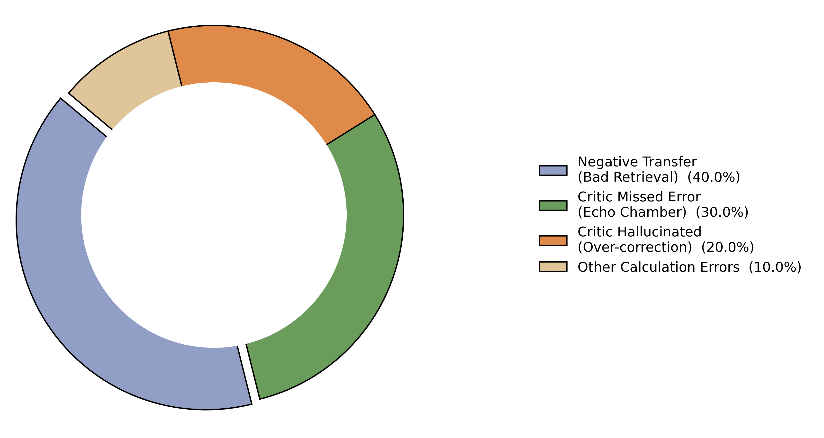
\includegraphics[width=0.78\linewidth]{figures/fig9_error_distribution.png}
  \captionof{figure}{Breakdown of failure modes in the remaining incorrect instances.}
  \label{fig:error_typology}
\end{center}

These observations suggest that developing richer confidence features for the Learned Selector and introducing more diverse, heterogeneous models for the Critic role are promising directions for future work.
